\documentclass[a4paper,12pt]{article}
\usepackage[utf8]{inputenc}
\usepackage[T1]{fontenc}
\usepackage{setspace} % This package is used to control linespacing; With \onehalfspacing for instance
\usepackage[danish]{babel}
\renewcommand{\danishhyphenmins}{22} % bedre orddeling
\usepackage{bm}
\usepackage{fnbreak}
\usepackage{sectsty}
\usepackage{wrapfig}
\usepackage[scriptsize]{caption}
\usepackage[danish,textsize=tiny,backgroundcolor=red,bordercolor=blue]{todonotes}
\usepackage[isbn,issn]{dk-bib}
\interfootnotelinepenalty=10000
\usepackage{graphicx}
\usepackage{usecases}
\usepackage{pdfpages}

\addto\captionsdanish{
\renewcommand\abstractname{Abstract}
}
%-----------------------------------------------------
\newcommand{\doctitle}{Assignment 1}
\newcommand{\docsubject}{02131 Embedded Systems}
\newcommand{\docauthor}{Cebrail, Jonathan og Christian}	
\newcommand{\docdate}{\today}
\newcommand{\docplace}{Danmarks Tekniske Universitet}
\newcommand{\HRule}{\rule{\linewidth}{0.5mm}}
%\newcommand{\docsubtitle}{Undertitle}
%-----------------------------------------------------

%-----------Scientific and mathematical packages begin-----------
% Math package
	\usepackage{amsmath}

% Vector symbols and functions (for example \vv)
	\usepackage{esvect}

% Mathematical symbols
	\usepackage{amssymb}
\DeclareMathOperator{\p}{\cdot}
\DeclareMathOperator{\N}{\mathbb{N}}
\DeclareMathOperator{\Z}{\mathbb{Z}}
\DeclareMathOperator{\C}{\mathbb{C}}
\DeclareMathOperator{\R}{\mathbb{R}}
\newcommand{\nn}{\nonumber}
% SI Units
	%\usepackage[output-decimal-marker={,}]{siunitx}		%http://mirrors.dotsrc.org/ctan/macros/latex/begincontrib/siunitx/siunitx.pdf
	%\sisetup{unitsep= \cdot }

% For Chemistry
	%\usepackage{chemscheme}		% http://ctan.org/pkg/chemscheme
	%\usepackage{chemsym}		% http://ctan.org/pkg/chemsym
	%\usepackage{mhchem}			% http://mirrors.dotsrc.org/ctan/macros/latex/contrib/chemstyle/chemstyle.pdf
	%\DeclareSIUnit\Molar{\textsc{m}}
%-----------Scientific and mathematical packages end--------------

% Non-default fonts - has to come _after_ some of the mathematical packages
\usepackage{pxfonts}

% Page margins
\usepackage[left=2.0cm, right=1.5cm]{geometry}

% Hyperref
\usepackage[colorlinks=true,linkcolor=black,citecolor=black,urlcolor=black]{hyperref}
%\usepackage[hidelinks]{hyperref}  
\hypersetup{pdftitle={\doctitle}} 
\hypersetup{pdfsubject={\docsubject}}
\hypersetup{pdfauthor={\docauthor}}

% Setspace
\usepackage{setspace}
\onehalfspacing
%\numberwithin{equation}{section}
% Alter some LaTeX defaults for better treatment of figures:
    % See p.105 of "TeX Unbound" for suggested values.
    % See pp. 199-200 of Lamport's "LaTeX" book for details.
    %   General parameters, for ALL pages:
    \renewcommand{\topfraction}{0.9}	% max fraction of floats at top
    \renewcommand{\bottomfraction}{0.8}	% max fraction of floats at bottom
    %   Parameters for TEXT pages (not float pages):
    \setcounter{topnumber}{2}
    \setcounter{bottomnumber}{2}
    \setcounter{totalnumber}{4}     % 2 may work better
    \setcounter{dbltopnumber}{2}    % for 2-column pages
    \renewcommand{\dbltopfraction}{0.9}	% fit big float above 2-col. text
    \renewcommand{\textfraction}{0.07}	% allow minimal text w. figs
    %   Parameters for FLOAT pages (not text pages):
    \renewcommand{\floatpagefraction}{0.7}	% require fuller float pages
	% N.B.: floatpagefraction MUST be less than topfraction !!
    \renewcommand{\dblfloatpagefraction}{0.7}	% require fuller float pages

	% remember to use [htp] or [htpb] for placement

% Title
\title{
\HRule \\
\textsc{\doctitle} \\
	 \small{\textsl{\docsubtitle}}
\HRule
}
\author{\docauthor\\\small{\docplace}}
\date{\docdate}

% Fancyheader : http://mirrors.dotsrc.org/ctan/macros/latex/contrib/fancyhdr/fancyhdr.pdf
\usepackage{fancyhdr}
\pagestyle{fancy}
\fancyhf{}
%\fancyhead[RO]{\docauthor \hfill \doctitle \hfill\thepage}
\fancyhead[RO]{\doctitle \hfill \docauthor \hfill \thepage /\ref{TotPages}}
% Get rid of annoying error messages
\setlength{\headheight}{14.5pt}
\usepackage{totpages}
\usepackage{sectsty}
\allsectionsfont{\scshape}
\begin{document}
\begin{titlepage}
\begin{center}
\textsc{\LARGE Danmarks Tekniske Universitet}\\[1.5cm]
\textsc{\large Embedded Systems 02131}\\[0.5cm]
\HRule \\[0.4cm]
{ \huge \bfseries Assignment 1}\\[0.1cm]
\HRule \\[1.5cm]
\end{center}
\begin{flushleft} \large
\emph{Gruppemedlemmer:}\\
Cebrail \textsc{Erdogan} s113414\\
Christian Mathias Rohde \textsc{Kiær} s123812\\
Jonathan Binner \textsc{Becktor} s123094\\
\end{flushleft}
\vfill 
\begin{center}
{\large \today}
\end{center}
\end{titlepage}
\newpage
\section*{Introduktion}
Vi har fået stillet til opgave at implementere Pan-Thompkins QRS detection algorithm. Algoritmens formål er at analysere et ECG signal og QRS komplekset. QRS komplekset giver det elektriske billede af ventriklernes sammentrækning. Et eksempel på et QRS kompleks ses på figur 1.\\
\begin{figure}[htp]
\centering
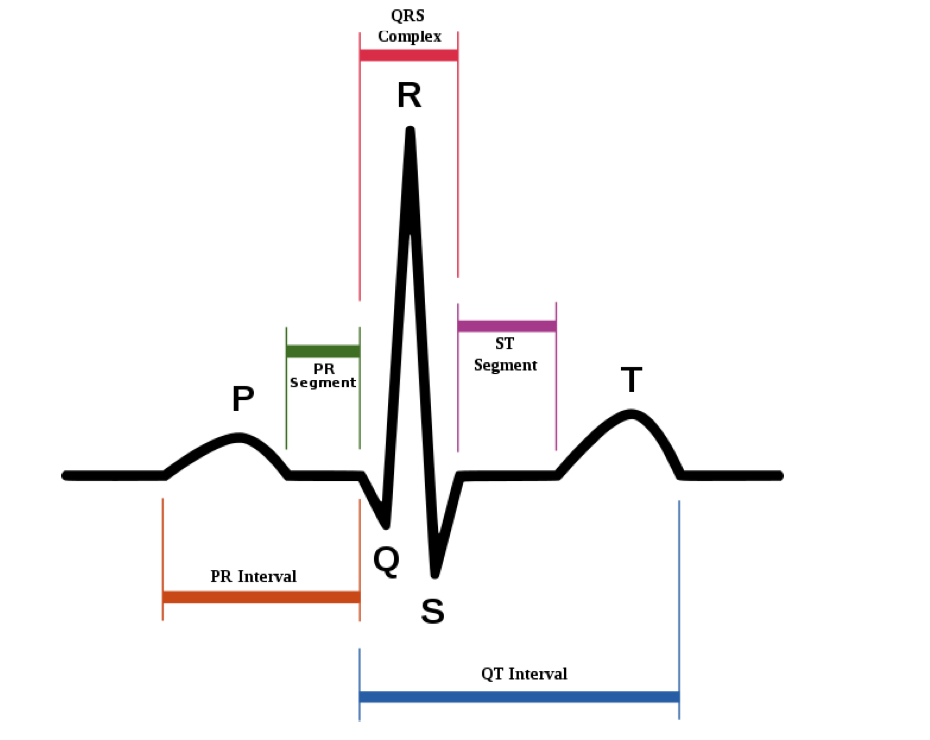
\includegraphics[scale=0.5]{qrs.png}
\caption{QRS Kompleks}
\label{Figur 1: QRS}
\end{figure}\\
Vores mål med algoritmen er derfor at give en vurdering af R peaks i QRS komplekset. Dette vil kunne alamere patienter om eventuelle hjerteproblemer. Vores algoritme skal derfor kunne registrere følgende:
\begin{itemize}
\item Intensiteten af R-peaks.
\item Varigheden af R-peaks.
\item Tiden siden sidste R-peak.
\item Advare hvis intensiteten af R-peaket er under en vis grænse eller hvis intervallet mellem R-peaks er ustabilt.
\end{itemize}
\newpage
\tableofcontents
\newpage
\section{Kravspecifikationer}
Vi vil her beskrive kravene for programmet, 
\subsection{Funktioner}
\subsubsection{Data erhvervelse}
Vores program skal kunne simulere en ECG måling. Der skal derfor indlæses et datasæt, som representere data fra en rigtigt patient, i realtime for så nøjagtigt som muligt at simulere en ECG måling.  
\subsubsection{Filtrering}
Da algoritmen kræver at datapunkterne behandles med stor præcision, anvendes 5 forskellige algoritmer til at filtrere den data vi har fået. De forskellige algoritmer gør alle noget forskelligt og meget spesefikt for datapunkterne. Low-Pass filtrer som i navnet lader de lave frekvenser komme forbi og blokerer de alt for høje. Highpass gør det modsatte. Derivative forstærker de signaler vi er interesseret i. Square filtrer tildeles for at vise større forskel mellem datapunkterne og for at gøre alle datapunkterne positive. Tilsidst bruges Moving window implementation filtret for at gøre signalet mere "blødt" altså at fjerne ekstra støj for at fobredre visualiseringen af R-peaks. De 5 filtre skal anvendes i følgende orden:
\begin{itemize}
\item Low-pass filter
\item High-pass filter
\item Derivative
\item Squaring
\item Moving window integration
\end{itemize}
\newpage

\subsection{Varierende del??}
\subsection{Bruger output??}
\section{Programdesign}
\subsection*{Struktur}
Vi har taget udgangspunkt i de udleverede program filer til senoren, og efterfølgende oprettet klasser for alle filtre og QRS-registrings delene af programmet. Vi har en main klasse der kører selve programmet, og derfra kalder de nødvændige funktioner.\\
Filtrene er oprettet med navn, og funktionerne i det pågældende filter bliver derfra kaldt (eks. er low-pass filteret oprettet som lowPass.c). R-peak registrering forgår i QRS.c, hvorfra også udregningerne af intensiteten, varigheden og tiden siden sidste R-peak foregår.\\
Opdelingen er sket på denne måde, da vi synes en klasse for hver filter gav mest overskuelighed. Det er meget let derfra at gå ind og rette på en enkelt del af et givent filter, uden det giver problemer i resten af programmet. At holde QRS funktionerne adskildt fra resten af programmet giver samme fordele. Nedenfor ses et klassediagram for vores program.
\begin{figure}[htpb]
\centering
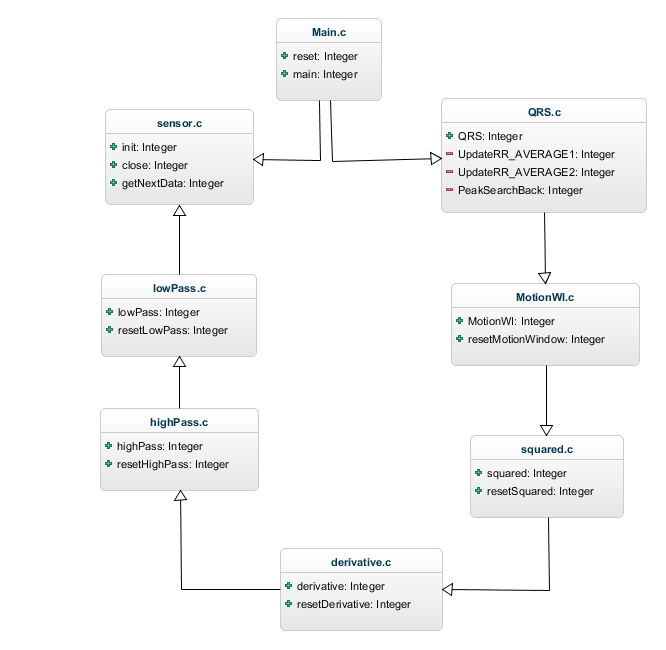
\includegraphics[scale=0.5]{fisse.jpg}
\caption{Klassediagram}
\label{Figur 2. Klassediagram}
\end{figure}
\newpage
\subsection{Data indlæsning}
Da programmet skal forestille at være en simulation af en ECG måling, ved brug af Pan-Thompsons QRS detection algorithm, skal programmet kunne læse data fra en fil. Til dette har vi vidreudviklet på sensor.c filen, og implenteret funktionen getNextData(). Dette vil give os muligheden for at hente data fra en fil, og bruge dette datasæt til analyse af QRS detection algoritmen. Sensor.c bruges derefter i main.c og henter alle vores signal data ind til analysen.
\subsection{Data analyse}
Analyseringen af data sker, når hver 
\subsection{Data output}
\section{Implementering}
\subsection{Filtre}
De forskellige filtre er belvet implementeret i hver sin klasse. Her er en gennemngang af nogle af dem da nogle af dem er meget ens hvor det eneste der gør dem forskellige er den matematiske formel.

\subsubsection{Low-Pass, High-pass, Derivative og Moving window implementation}
Her initializeres 2 arrays en til resultaterne og en til dataen. Størrelsen af arrayet afhænger af hvor langt tilbage formlen siger vi skal have resultater fra. Fx. skal vi have $x_{n-12}$ i Low-Pass filtret, vi skal altså have et array der gemmer x værdierne til og med $x_{n-12}$. Det bliver gjort med en forløkke som sætter den positon næste lig den forrige.
Hvorefter vi så returner resultatet. Derudover har vi også tilføjet en reset metode hvis man skal bruge filtrene igen. Den sætter bare alle positionerne i arraysne til nul.
\subsection{QRS Detection algorithm}


QRS algoritmen er uden tvivl den vigtigste komponent i hele systemet. Den har til formål at finde ”peaks” – altså toppe – og behandle de fundne peaks. Algoritmen gør det muligt at fortolke frekvenserne. Nogle af de fundne peaks vil blive fortolket som hjertepuls (Rpeaks), mens nogle af dem fortolkes som støj. Hvis intervallet mellem Rpeaks er usædvanligt vil programmet kommet med output - advarelser. De essentielle dele af algoritmen bliver uddybet nedenfor.
\subsubsection{peaks}
Peaks er simple at finde. Der hentes data fra filteret. De hentes en ad gangen, men man kunne også hente tre ad gangen. Grunden til at der skal bruges tre ”datapoint” skyldes betingelsen:
$Xn-1 < xn, xn > xn+1$  ,  
Gemme peaks
Peaks er defineret som ”struct”. Struct gør det muligt at oprette et object og give den forskellige variabler. Så alle vores peaks har variablerne ”value”,”RR” og ”index”.
Nu er peak en type som kan tildeles. De fundne peaks gemmes i et array med typen peak. 

\subsubsection{RR intervallet}

Intervallet af Rpeaks afgøre patientens tilstand, derfor er det også dem der bruges til at de forskellige udsagn i algoritmen. Vi beregner intervallet ved at sige:
Datapoint\_index  - index of last $Rpeak = interval$
Hvis RR intervallet ligger mellem RR\_LOW og RR\_HEIGHT er der intet galt, men hvis dette viser sig ikke at være tilfældet i 5 gange i træk, vil programmet komme med en advarsel. De seneste RR intervaller gemmes i en array med størrelsen 8, de fundne bruges til at finde gennemsnittet.

Søg baglæns for peaks
Når intervallet ikke er mellem RR\_LOW og RR\_HEIGHT vil den blive tjekket om den er større end RR\_MISS, hvis det er tilfældet vil den starte proceduren ”searchback”. 
I ”searchback” gennemsøger vi baglæns gennem alle de fundne ”peaks” indtil videre.
Lige så snart vi har en peak som er større end THRESHOLD2 fortsætter vi til algoritmens sidste step. Hver gang der betingelsen ikke er opfyldt går vi en skridt tilbage i arrayet.
 

\subsubsection{Squared}
Squared filtret ligger også i sin egen klasse. her får den input fra Derivative og returner inputtet ganget sig selv.

\section{Resultater}
Resultaterne er som ventet når "patienten" har problemer med hjertet får vi en advarsel og vi finder alle andre Rpeaks. Derudover kan vores program køre den store liste ECG10800K på 2.4sec, og vi har fået en average run time på ?????(HURTIG).
\begin{figure}[htp]
\centering
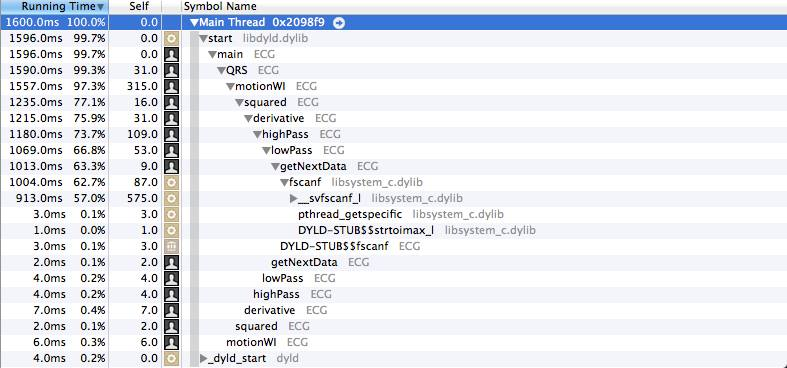
\includegraphics[scale=0.6]{CPUperformance.jpg}
\caption{CPU performance chart ved brug af ECG10800K.txt}
\label{CPU performance chart ved brug af ECG10800K.txt}
\end{figure}
\section{Diskussion}
Vi som gruppe havde alle lavet en forskellig version af programmet og så senere merget det og fået et program som virker som det skal. Vi var i tvivl hvordan vi skulle håndtere alle de forskellige variabler der ville komme og havde rigtigt mange store arrays sat op, vi fant dog ud af at bruge structs for at have noget der minder objekter.
\section{Konklusion}
\newpage
\section{Bilag}
\subsection{HelloWorld.c}
\begin{verbatim}
#include <stdio.h>

int main(int argc, const char * argv[])
{
    printf("Hello, World!\n");
    return 0;
}
\end{verbatim}
\subsection{ReadFile.c}
\begin{verbatim}
#include <stdio.h>

int main(int argc, const char * argv[])
{
    static const char filename[] = "/users/christiankiaer/Downloads/ECG.txt";
    FILE *file = fopen ( filename, "r" );
    
    int maxReading;
    int i1;
    while (fscanf(file,"%i",&i1) != EOF)
    {
        if (i1 > maxReading)
        {
            maxReading = i1;
        }
    }
    
    printf("The highest EKG reading is: %i", maxReading);
    return 0;
}
\end{verbatim}
\end{document}